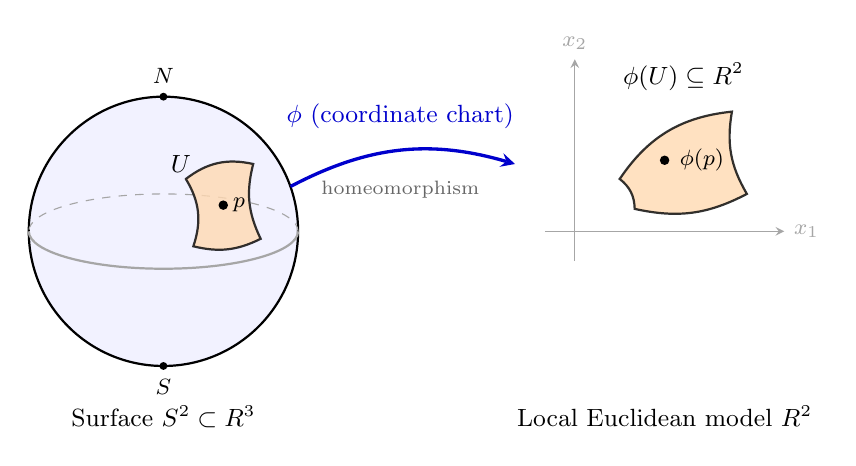
\begin{tikzpicture}[scale=0.95, >=stealth]
  % Left: Sphere S^2
  \begin{scope}[shift={(0,0)}]
    % Sphere outline
    \draw[thick, fill=blue!5] (0,0) circle (1.8);
    % Equator (front solid, back dashed)
    \draw[dashed, gray!70] (1.8,0) arc (0:180:1.8 and 0.5);
    \draw[thick, gray!70] (-1.8,0) arc (180:360:1.8 and 0.5);
    % North and South labels
    \node[above, font=\footnotesize] at (0, 1.85) {$N$};
    \fill (0,1.8) circle (1.5pt);
    \node[below, font=\footnotesize] at (0, -1.85) {$S$};
    \fill (0,-1.8) circle (1.5pt);

    % Local open patch U on sphere
    \draw[thick, fill=orange!30, opacity=0.8] 
      (0.3, 0.7) to[bend left=25] (1.2, 0.9) 
      to[bend right=20] (1.3, -0.1) 
      to[bend left=20] (0.4, -0.2) 
      to[bend right=25] cycle;
    \node[above left, font=\small] at (0.5, 0.65) {$U$};
    \fill (0.8, 0.35) circle (1.8pt) node[right, font=\footnotesize] {$p$};
    \node[below, font=\small] at (0, -2.2) {Surface $S^2 \subset \mathbb{R}^3$};
  \end{scope}

  % Middle: Coordinate chart map phi
  \draw[->, very thick, blue!80!black] (1.7, 0.6) to[bend left=22] 
    node[above=4pt, font=\small] {$\phi$ (coordinate chart)} 
    node[below=7pt, font=\scriptsize, text=gray!80!black] {homeomorphism} (4.7, 0.9);

  % Right: Flat open set in R^2
  \begin{scope}[shift={(5.5,0)}]
    % Axes - crossing at (0,0), clear of the region
    \draw[->, gray!70, thin] (-0.4, 0) -- (2.8, 0) node[right, font=\footnotesize] {$x_1$};
    \draw[->, gray!70, thin] (0, -0.4) -- (0, 2.3) node[above, font=\footnotesize] {$x_2$};
    
    % Flat open region phi(U) placed cleanly in the positive quadrant away from axes
    \draw[thick, fill=orange!30, opacity=0.8] 
      (0.6, 0.7) to[bend left=25] (2.1, 1.6) 
      to[bend right=20] (2.3, 0.5) 
      to[bend left=20] (0.8, 0.3) 
      to[bend right=25] cycle;
      
    % Region label placed comfortably above
    \node[above, font=\small] at (1.45, 1.75) {$\phi(U) \subseteq \mathbb{R}^2$};
    
    % Point phi(p) with label placed centered horizontally inside the orange patch
    \fill (1.2, 0.95) circle (1.8pt) node[right=2pt, font=\footnotesize] {$\phi(p)$};
    
    \node[below, font=\small] at (1.2, -2.2) {Local Euclidean model $\mathbb{R}^2$};
  \end{scope}
\end{tikzpicture}
